%%%%%%%%%%%%%%%%%%%%%%%%%%%%%%%%%%%%%%%%%%%%%%%%%%%%%%%%%%%%%%%%%%%%%%%%%%%%%%%%%
% This is the source for a C Style Guide by Ethan Ruffing.
%
% Copyright 2015-2016 by Ethan Ruffing
%%%%%%%%%%%%%%%%%%%%%%%%%%%%%%%%%%%%%%%%%%%%%%%%%%%%%%%%%%%%%%%%%%%%%%%%%%%%%%%%%

\documentclass[11pt]{book}
\usepackage{amssymb,amsmath}
\usepackage{caption}
\usepackage{appendix}
\usepackage{float}
\usepackage{pdfpages}
\usepackage{amsmath}
\usepackage{amssymb}
\usepackage{enumitem}
\usepackage{cclicenses}
\usepackage{fancyhdr}

% Comment the following line to use Computer Modern typeface, uncomment to use
% Times and Courier
%\usepackage{times}

% Defined to allow numbering of one line in an `align` environment
\newcommand\numberthis{\addtocounter{equation}{1}\tag{\theequation}}

% Use the following to configure the page geometry
\usepackage[letterpaper, portrait]{geometry}

% The following line changes from indenting paragraphs to placing blank lines
% between them
\usepackage{parskip}
\setlist[itemize]{parsep=0pt}

% Set up settings for listings
\usepackage{listings}
\usepackage{color}
\definecolor{mygreen}{rgb}{0,0.6,0}
\definecolor{mygray}{rgb}{0.5,0.5,0.5}
\definecolor{mymauve}{rgb}{0.58,0,0.82}
\lstset{
	% Choose the background color; you must add \usepackage{color} or
	% \usepackage{xcolor}
	backgroundcolor=\color{white},
	% The size of the fonts that are used for the code
	basicstyle={\ttfamily},
	% Sets if automatic breaks should only happen at whitespace
	breakatwhitespace=false,
	% Sets automatic line breaking
	breaklines=true,
	% Sets the caption-position to bottom
	captionpos=b,
	% Comment style
	commentstyle=\color{mygreen},
	% If you want to delete keywords from the given language
	deletekeywords={...},
	% If you want to add LaTeX within your code
	%escapeinside={\%*}{*)},
	% Lets you use non-ASCII characters; for 8-bits encodings only, does not work
	% with UTF-8
	extendedchars=true,
	% Adds a frame around the code
	frame=single,
	% Keeps spaces in text, useful for keeping indentation of code (possibly needs
	% columns=flexible)
	keepspaces=true,
	% Keyword style
	keywordstyle=\color{blue},
	% The language of the code (can be overriden on individual listings)
	language=C,
	% If you want to add more keywords to the set
	otherkeywords={...},
	% Where to put the line-numbers; possible values are (none, left, right)
	numbers=left,
	% How far the line-numbers are from the code
	numbersep=5pt,
	% The style that is used for the line-numbers
	numberstyle=\tiny\color{mygray},
	% If not set, the frame-color may be changed on line-breaks within not-black
	% text (e.g. comments (green here))
	rulecolor=\color{black},
	% Show spaces everywhere adding particular underscores; it overrides
	% 'showstringspaces'
	showspaces=false,
	% Underline spaces within strings only
	showstringspaces=false,
	% Show tabs within strings adding particular underscores
	showtabs=false,
	% The step between two line-numbers. If it's 1, each line will be numbered
	stepnumber=2,
	% String literal style
	stringstyle=\color{mymauve},
	% Sets default tabsize to 2 spaces
	tabsize=4,
	% Show the filename of files included with \lstinputlisting; also try caption
	% instead of title
	title=\lstname
}
% Use the {code} environment instead of the {lstlisting} environment to prevent
% breaking across pages. All other options and properties will be the same.
\lstnewenvironment{code}[1][]%
	{\noindent\minipage{\linewidth}\medskip
		\lstset{basicstyle=\ttfamily\footnotesize,frame=single,#1}}
	{\endminipage}

% Set up hyperref package (used for cross-references)
\usepackage{hyperref}
\hypersetup{
    colorlinks,
    citecolor=black,
    filecolor=black,
    linkcolor=black,
    urlcolor=black
}
\def\chapterautorefname{Section}

\fancypagestyle{numberingAndCC}{
	\fancyhf{}
}

\usepackage{url}
\renewcommand{\theenumi}{\alph{enumi}} \renewcommand{\theenumii}{\arabic{enumii}}
	\renewcommand{\labelenumii}{\theenumii.}
\usepackage{adjustbox}

\def\secondpage{\clearpage\null\vspace*{0.2\textheight}
	\pagestyle{empty}
	\begin{minipage}[t!]{0.9\textwidth}
		Copyright \copyright 2014--\the\year\ by Ethan Ruffing.\par
		
		\begin{figure}[H]
			\includegraphics[scale=0.9]{by-nc-nd.eps}
		\end{figure}
		
		This work is licensed under the Creative Commons
		Attribution-NonCommercial-NoDerivatives 4.0 International License. To
		view a copy of this license, visit
		\url{http://creativecommons.org/licenses/by-nc-nd/4.0/}.
	\end{minipage}
	\vspace*{4\baselineskip}
	\cleardoublepage
}

\makeatletter
\g@addto@macro{\maketitle}{\secondpage}
\makeatother


% The following section makes everything get numbered by section. Comment out to
% return to normal numbering.
\usepackage{chngcntr}
\AtBeginDocument{
	\counterwithin{equation}{chapter}
	\counterwithin{figure}{chapter}
	\counterwithin{table}{chapter}
	\counterwithin{lstlisting}{chapter}
}

\title{C Style Guide}
\date{\today}
\author{Ethan Ruffing}

\begin{document}

% Create title page
\begin{titlepage}
	\maketitle
	\thispagestyle{empty}
\end{titlepage}
\pagenumbering{roman} % Number pages i, ii, ...

% Generate table of contents
\tableofcontents

\newpage
\pagenumbering{arabic} % Number pages 1, 2, ...

\chapter{Introduction}\label{ch:introduction}
When programming, it is essential for all programmers on a project to follow a
common style. Doing so ensures consistency and productivity, allowing for a
final product which is better functioning and more appealing to the client.
A consistent style and detailed documentation will allow colleagues and future
programmers to easily understand and use new source code.

This style guide is intended to provide a unifying basis for programming in the
C programming language, and to provide a standard for documenting the programs
created.

\chapter{File \& Program Organization}\label{ch:file-program-organization}

\section{File Format}\label{sec:file-format}

Source code should be written so that no line exceeds eighty characters
in length.

A header block should be placed at the top of each file giving the
author, the date of creation, and, if applicable, the version number.
This header block should also include a copyright notice and license
header if applicable.

File names should be clear and concise so that someone can tell the
general purpose of the file without having to open and read it or its
header block.

\section{File Structure}\label{file-structure}

Function \emph{declarations} should always be located within a header
(\texttt{*.h}) file, while function \emph{definitions} should be located
in a source (\texttt{*.c}) file. If choosing to place documentation for
the function in only one of these locations, it is best to place it in
the header file, as the header file is intended to contain a high-level
overview of each function.

\section{Program Structure}\label{program-structure}

Every effort should be made to avoid the use of global variables.
Instead, pre-processor macros should be used for constants, and
variables should be passed and returned between functions.

\chapter{Commenting \& Documentation}\label{commenting-documentation}

\section{Comments}\label{comments}

Comments should be included where necessary to give a better
understanding of code. When writing longer comments, follow Strunk \&
White's \emph{The Elements of Style} for English grammar guidelines.

When writing dates and times, use the ISO 8601 standard. That is, for
dates, YYYY-MM-DD; for times, hh:mm:ss; and, for date-times,
YYYY-MM-DDThh:mm:ss.

Comments should be included that give detailed descriptions of all
functions, classes, and instance variables.

\section{Program Documentation}\label{program-documentation}

It is essential to provide a brief overview of your program. Such an
overview should be placed in a file named \texttt{README.md}, and
formatted using Markdown (a markup language designed to create
nicely-formatted, but still easily parsed, plain-text files). This file
should contain an overview of the program's purpose, its authors, and
relavent copyright information. It should also include directions on
where to find more extensive documentation, for both users and
developers. However, detailed documentation on the program's
functionality should \emph{not} be included in this file.

In addition, it is prudent to maintain a \texttt{CHANGELOG} (or, if
preferred, \texttt{CHANGELOG.md}) file, in which a brief overview of the
changes made between each release of the program are listed. Note that
the changes listed here should be only the major differences between
versions; all minor changes and modifications should be recorded using
some form of version control, such as Git or SVN.

\section{Function Documentation}\label{function-documentation}

DocBlock-style comments should be provided for \emph{every} function.
DocBlock comments should be formatted using the \texttt{/**\ ...\ */}
system, as illustrated in \autoref{lst:doxygen-example}.

The most commonly used DocBlock interpreter for C documentation is
\href{http://www.stack.nl/~dimitri/doxygen/}{Doxgen}. It supports export
into a multitude of formats and supports a large number of tags. For a
reference of what tags are supported, see the
\href{http://www.stack.nl/~dimitri/doxygen/manual/commands.html}{Special
Commands} section of the
\href{http://www.stack.nl/~dimitri/doxygen/manual/index.html}{Doxygen
Manual}.

Author and date (or \texttt{@since}) should \emph{always} be given for a
file DocBlock. If using version numbering for the project, the version
tag (showing the current version number, not that at which the file was
introduced) should also \emph{always} appear in the file DocBlock.

At a minimum, functions should \emph{always} have the \texttt{@date} (or
\texttt{@since}) tags. If multiple authors have contributed to the same
file, then each function's block \emph{must} include an \texttt{@author}
tag, as well. (If not given, the author is to be assumed to be the same
as the file author.)

Functions should also have \texttt{@param} and \texttt{@return} tags
where applicable. Parameter tags should specify the parameter direction
(\texttt{{[}in{]}} or \texttt{{[}out{]}}, as seen in the example below).
The description portion of these tags should be located on the next line
(after the tag and variable name) and indented one level past the tag
itself.

If absolutely necessary to use, global variables should have a DocBlock
comment to explain their purpose. Macros should be described in a block
somewhere near the beginning of the file (though not in the file's
description/header block).

Description text should be written in sentences and be punctuated with a
period. Variable and \texttt{@param}/\texttt{@return} value
descriptions, however, should be kept brief and not written as full
sentences, unless absolutely necessary. (The first letter of these
descriptions, though, should still be capitalized.)

A blank line should be placed after each paragraph of explanation;
between the explanation and author, date, and version tags; and between
those tags and the \texttt{@param} and \texttt{@return} tags. (Note,
however, that there should \emph{not} be a blank line between
\texttt{@param} and \texttt{@return} tags.)

\begin{code}[caption=Example of Doxygen comments.,label=lst:doxygen-example]
/**
 * This is an explanation of a function.
 *
 * @author Ethan Ruffing <ruffinge@gmail.com>
 * @since 2014-08-06
 *
 * @param[in] varName
 *     A brief description of the parameter varName
 * @param[out] outName
 *     A brief description of the output outName
 * @return
 *     A brief description of the function's return value
 */
char doSomething(int varName, int *outName) {
    *outName = varName + 1;
    return varName % 2 == 0 ? 'y' : 'n';
}
\end{code}

\chapter{Basic Formatting}\label{basic-formatting}

C source files should be written according the the Kernighan and Ritchie
(K \& R) style. Furthermore, source files should be written according to
the C11 (ISO/IEC 9899:2011) standard. Extensive documentation on both of
these can be found online.

\section{Naming}\label{naming}

In general, names should be concise, but long enough to understand
immediately.

The following rules are non-negotiable with regards to the case used for
names.

\subsection{Variables and Functions}\label{variables-and-functions}

All variables and functions should be named in
\texttt{headlessCamelCase}.

\subsection{Constants and Macros}\label{constants-and-macros}

Constants and pre-processor macros should be named in
\texttt{SCREAMING\_SNAKE\_CASE}.

\section{Whitespace}\label{whitespace}

Whitespace helps tremendously to improve readability. The following are
basic guidelines, but can be expanded on to further improve readability.

\subsection{Indentation}\label{indentation}

There seems to be an ongoing war regarding indentation in programming.
For the purposes of this style guide, we will require the use of hard
tabs (an actual \texttt{\textbackslash{}t} character). IDEs and text
editors should be set to use a tab width of four, and alignment of items
such as comments should be based on this assumption.

There is one exception to this rule (which was alluded to previously):
When formatting block comments, all text within the block should be
aligned using spaces in order to guarantee readable documentation
everywhere. (NOTE, however, that the comment block itself should be
indented using tabs.)

\subsection{Blank Lines}\label{blank-lines}

One blank line should always be used in the following locations:

\begin{itemize}
\item
  Between functions
\item
  Between a local variable in a function and its first statement
\item
  Before a block or single-line comment
\item
  Between logically separate sections of code within a function
\end{itemize}

\subsection{Blank Spaces}\label{blank-spaces}

Blank spaces should be used in the following locations in order to enhance
readability (an example is shown in \autoref{lst:spacing-example}):

\begin{itemize}
\item
  Between a keyword and a parenthesis. Note that a blank space should
  \emph{not} be used between a function and its opening parenthesis. Also,
  there should not be any blank space following an opening parenthesis
  or preceding a closing parenthesis.
\item
  Before an opening brace (see above example)
\item
  Between binary and ternary operators and their operands
\item
  \emph{Not} between unary operators and their operands
\item
  After each semicolon in a \texttt{for} loop
\end{itemize}

\begin{code}[caption=Spacing example, label=lst:spacing-example]
void example(int a) {
	int i, b = 2, c;
	for (i = 0; i < n; i++) {
		c = a + b;
		c = a ? b - 1 : b + 1;
	}
}
\end{code}

\subsection{Braces}\label{braces}

\begin{itemize}
\item
  All loops, conditionals, and other such structures where braces are
  functionally ``optional'' \emph{must} use braces, even if their
  contents is a single line.
\item
  Opening braces should always be on their own line, aligned on the
  column of the item they are for.
\item
  Close braces should always be on their one line, aligned horizontally
  with their open statement.
\end{itemize}

\chapter{Error Handling}\label{error-handling}

There are multiple existing systems of error handling. For example, one
established way to pass errors in C is to return ``error code'' values
as integers. When using this function, a \texttt{0} is considered a successful
return, and any other value is considered an error.

It is prudent to devise and follow and error handling and checking
system to use in all programs.

\end{document}
